\newpage
\setheaders{Keynote Speaker: Claudio Pinhanez}{\daydateyear}
\section{Keynote Speaker: Claudio Pinhanez}
\index{Pinhanez, Claudio}

\begin{center}
{\bfseries\Large Harnessing the Power of LLMs\\\vspace{2.0\lineskip}to Vitalize Indigenous Languages} \\
\vspace{1.0em}
{\large\bf Claudio Pinhanez} \\
IBM Research Brazil

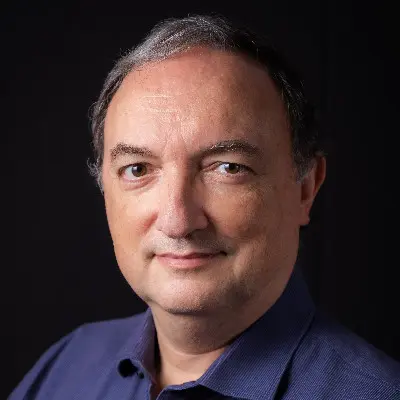
\includegraphics[width=0.4\linewidth]{content/day1/claudio-headshot.png}

\textbf{\daydateyear{}, 09:30--10:30 CST}\\
\textbf{\PlenaryLoc{}}
\end{center}

\noindent
{\bfseries Abstract:} How can Large Language Models (LLMs) and modern NLP be used to increase the use and the documentation of Indigenous languages which are in danger of disappearing? First, I report on the development of high-quality translators for Indigenous languages by fine-tuning SOTA machine translators with tiny amounts of data, and discuss how to avoid some common pitfalls. Next, I present prototypes built with Indigenous communities aiming to stimulate and facilitate writing, using LLM models to create spell-checkers, next-word predictors, and similar tools. Finally, I discuss a future for documentation where dying languages are preserved as interactive language models.

\vspace{1em}

{\bfseries Biography:} 
Claudio Pinhanez is a scientist, innovator, and professor. He is currently a Principal Scientist in the laboratory of IBM Research in Brazil where he leads research on artificial intelligence, human-machine interaction, and natural language processing. He is also the Deputy Director of the Center for Artificial Intelligence of the University of S\~ao Paulo, where he is a Visiting Professor at the Institute of Advanced Studies. Claudio got his Ph.D.~from the MIT Media Laboratory in 1999, joined the IBM Research T.J.~Watson laboratory in New York and in 2010 co-founded the IBM Research laboratory in Brazil. Since 2022 he leads a joint project of IBM Research and the University of S\~ao Paulo focused on the use of AI technology to document and vitalize Brazilian Indigenous languages.

\newpage
